\documentclass[a4paper,11pt,twoside]{article}
%\documentclass[a4paper,11pt,twoside,se]{article}

\usepackage{UmUStudentReport}
\usepackage{verbatim}   % Multi-line comments using \begin{comment}
\usepackage{courier}    % Nicer fonts are used. (not necessary)
\usepackage{pslatex}    % Also nicer fonts. (not necessary)
\usepackage[pdftex]{graphicx}   % allows including pdf figures
%\usepackage{lmodern}   % Optional fonts. (not necessary)
%\usepackage{tabularx}
%\usepackage{microtype} % Provides some typographic improvements over default settings
%\usepackage{placeins}  % For aligning images with \FloatBarrier
%\usepackage{booktabs}  % For nice-looking tables
%\usepackage{titlesec}  % More granular control of sections.

% DOCUMENT INFO
% =============
\department{Institution för Datavetenskap}
\coursename{Datavetenskapens byggstenar 7.5 p}
\coursecode{DV160HT15}
\title{OU3 Tables}
\author{Lorenz Gerber  ({\tt{dv15lgr@cs.umu.se}})}
\date{2015-12-17}
%\revisiondate{2015-09-15}
\instructor{Lena Kallin Westin / Johan Eliasson}


% DOCUMENT SETTINGS
% =================
\bibliographystyle{plain}
%\bibliographystyle{ieee}
\pagestyle{fancy}
\raggedbottom
\setcounter{secnumdepth}{2}
\setcounter{tocdepth}{2}
%\graphicspath{{images/}}   %Path for images

% DEFINES
% =======
%\newcommand{\mycommand}{<latex code>}


% DOCUMENT
% ========
\begin{document}
\maketitle

\tableofcontents
\newpage

\section{Introduction} 
Introduction 1/4 to 1 page. Describe with own words the aim and what
was done. Include also a description of the abstract data type
`table', and or reference \cite[po. 117 -- 132]{janlert2000}.

\section{Material and Methods} 
Describe the construction of the datatypes. 1/2 to 2 pages. This
should further include:
\begin{itemize}
\item how the implementations handle the case taking away non existing
  key
\item how the implementations handle double keys
\item proposing changes in the interface
\item why can we not use key as index in ArrayTable
\end{itemize}

Two test sets were provided, one to asses correctness of
implementation, the other to benchmark the speed for some typical
operations. 

Correctness of the data types was assessed by eight
differnt tests: 
\begin{itemize}
\item `isEmtpy' on a new created table yields TRUE
\item insert a single element
\item lookup a single element
\item insert and lookup multiple elements with non identical keys
table
\item insert and lookup multiple elements with identical keys
\end{itemize}

The benchmarks included five different cases: 
\begin{itemize}
\item Insert speed
\item random existing lookup speed
\item random non-existing lookup speed 
\item skewed lookup speed
\item remove speed  
\end{itemize}

\section{Results}
Present the results of the testing (1-2 pages, graphs/tables not
included). Include the testparameters with the presentation of the
results.
\begin{figure}[H] 
\centering 
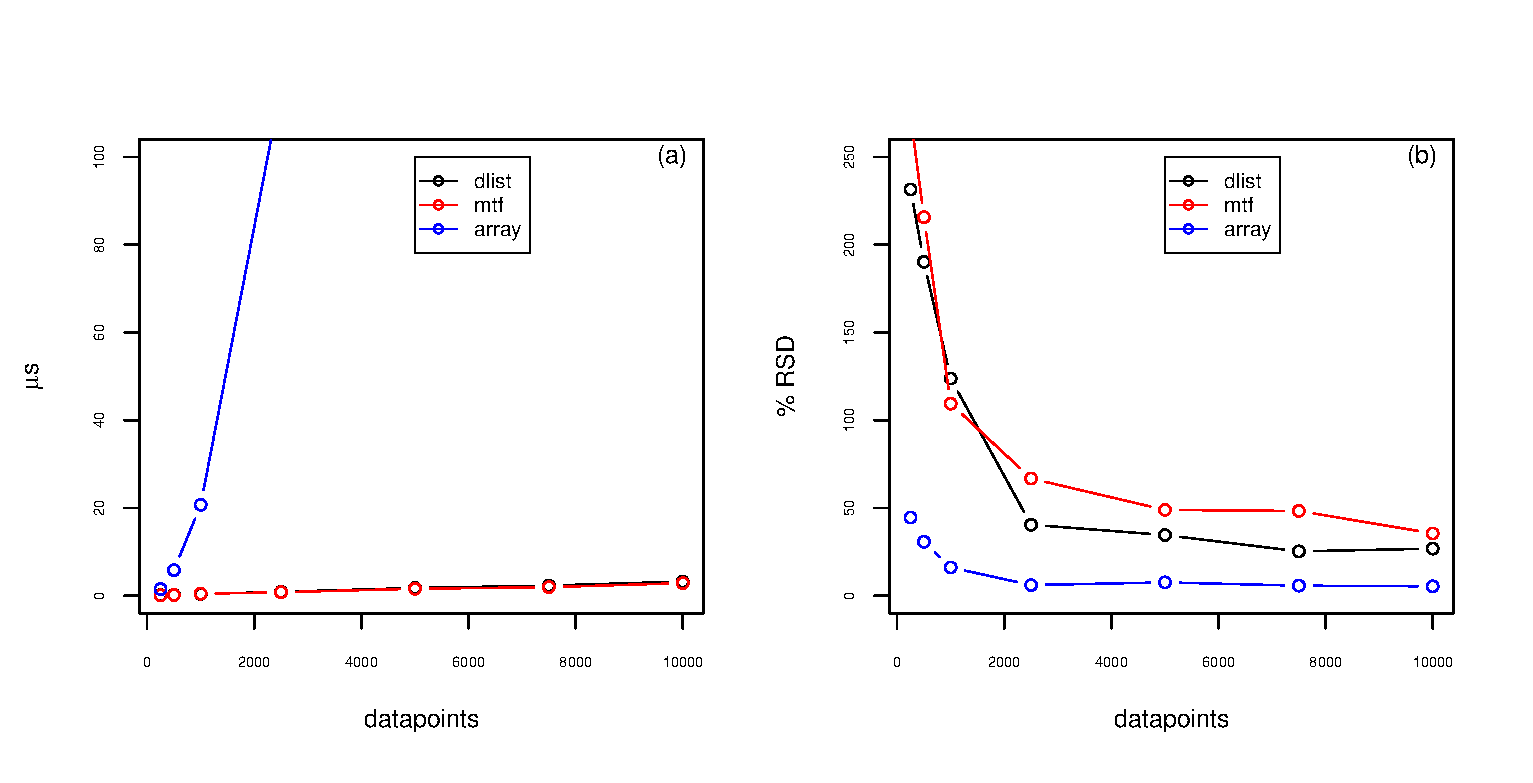
\includegraphics[width=\textwidth]{figures/fig1.eps}
\caption{\textit{Figure 1a, shows the element \textbf{`insertion'}
    times. Figure 1b shows the RSDs from the measurments in figure 1a. n=10.}}
\end{figure}

\begin{figure}[H] 
\centering 
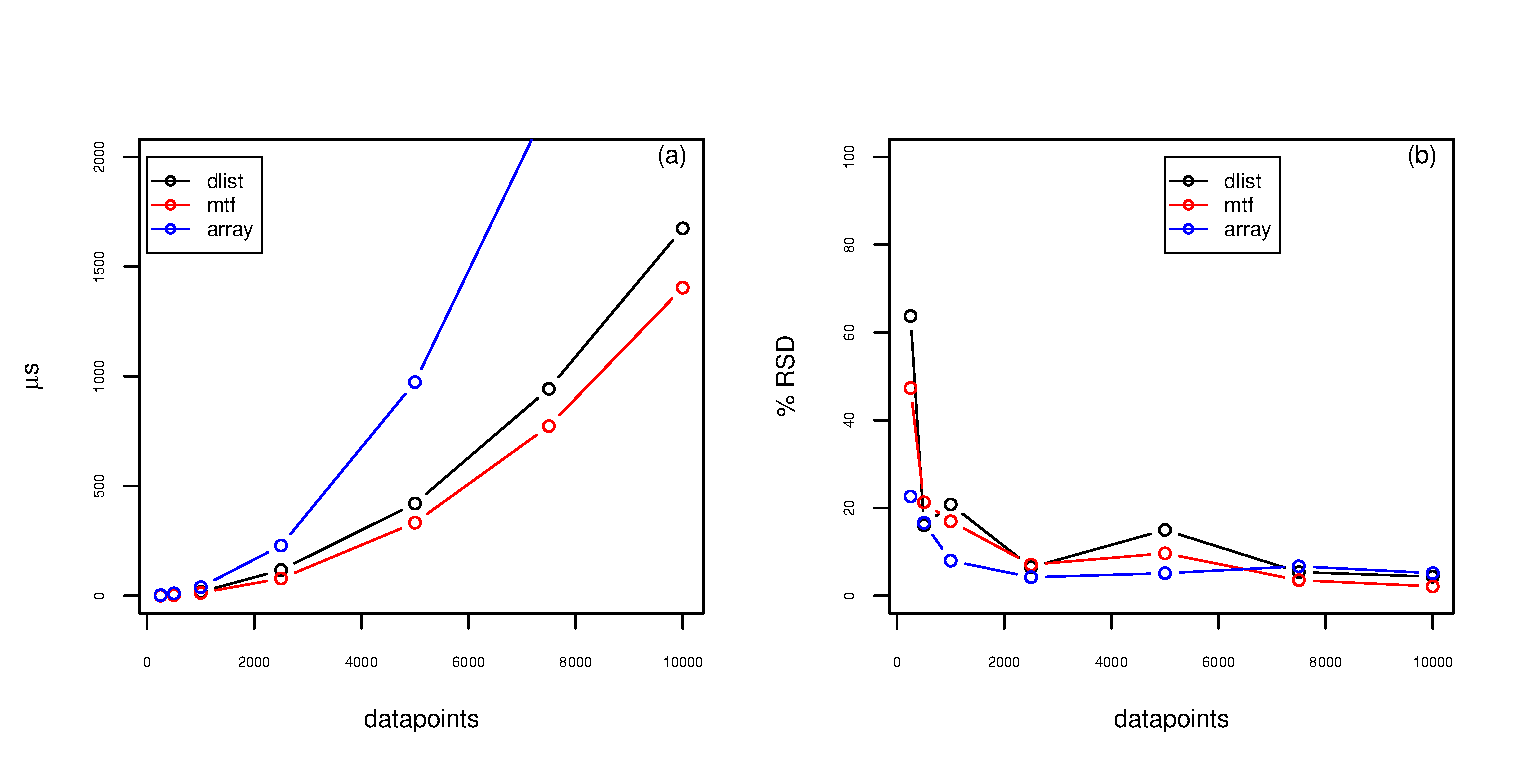
\includegraphics[width=\textwidth]{figures/fig2.eps}
\caption{\textit{Figure 2a, shows the times for the \textbf{`Random Existing
    Lookup'} benchmark. Figure 2b shows the RSD's from the measurments
in figure 2a. n=10.}}
\end{figure}

\begin{figure}[H] 
\centering 
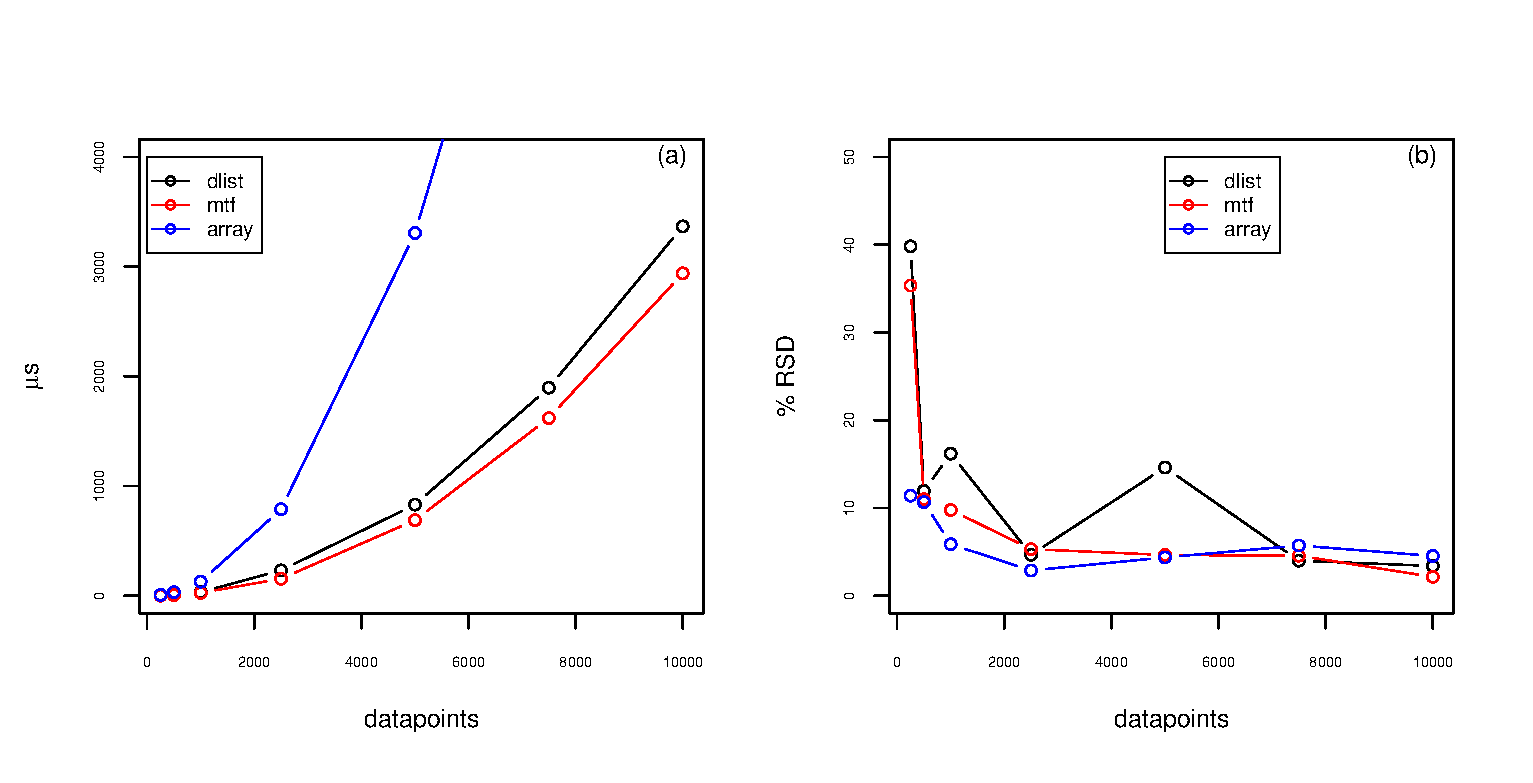
\includegraphics[width=\textwidth]{figures/fig3.eps}
\caption{\textit{Figure 3a, shows the times for the \textbf{`Random
      Non-Existing Lookup'} benchmark. Figure 3b shows the RSD's from
    the measurments in figure 3a. n=10.}}
\end{figure}

\begin{figure}[H] 
\centering 
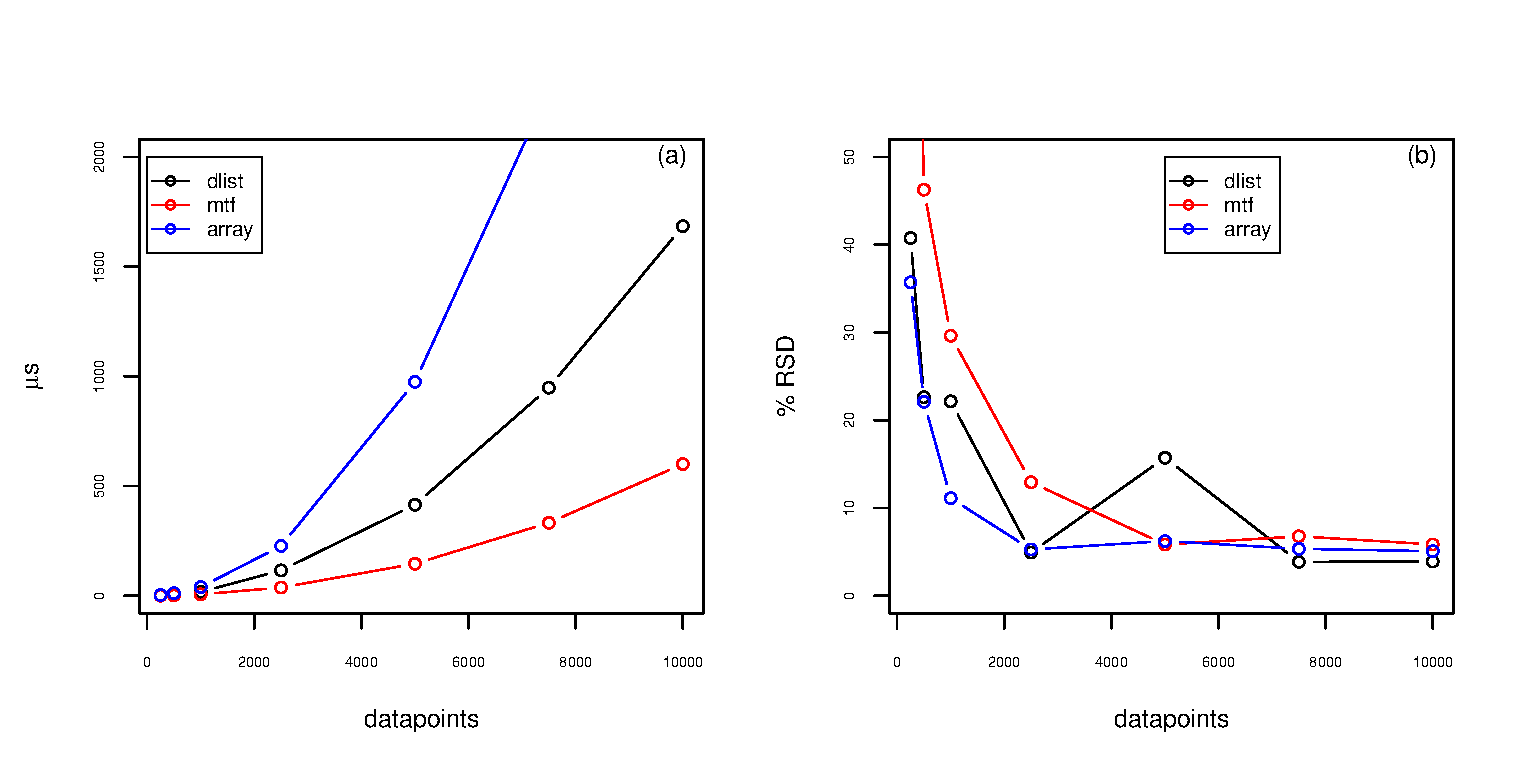
\includegraphics[width=\textwidth]{figures/fig4.eps}
\caption{\textit{Figure 4a, shows the times for the \textbf{`Skewed
      Lookup'} benchmark. Figure 4b shows the RSD's from the
    measurments in figure 4a. n=10.}}
\end{figure}

\begin{figure}[H] 
\centering 
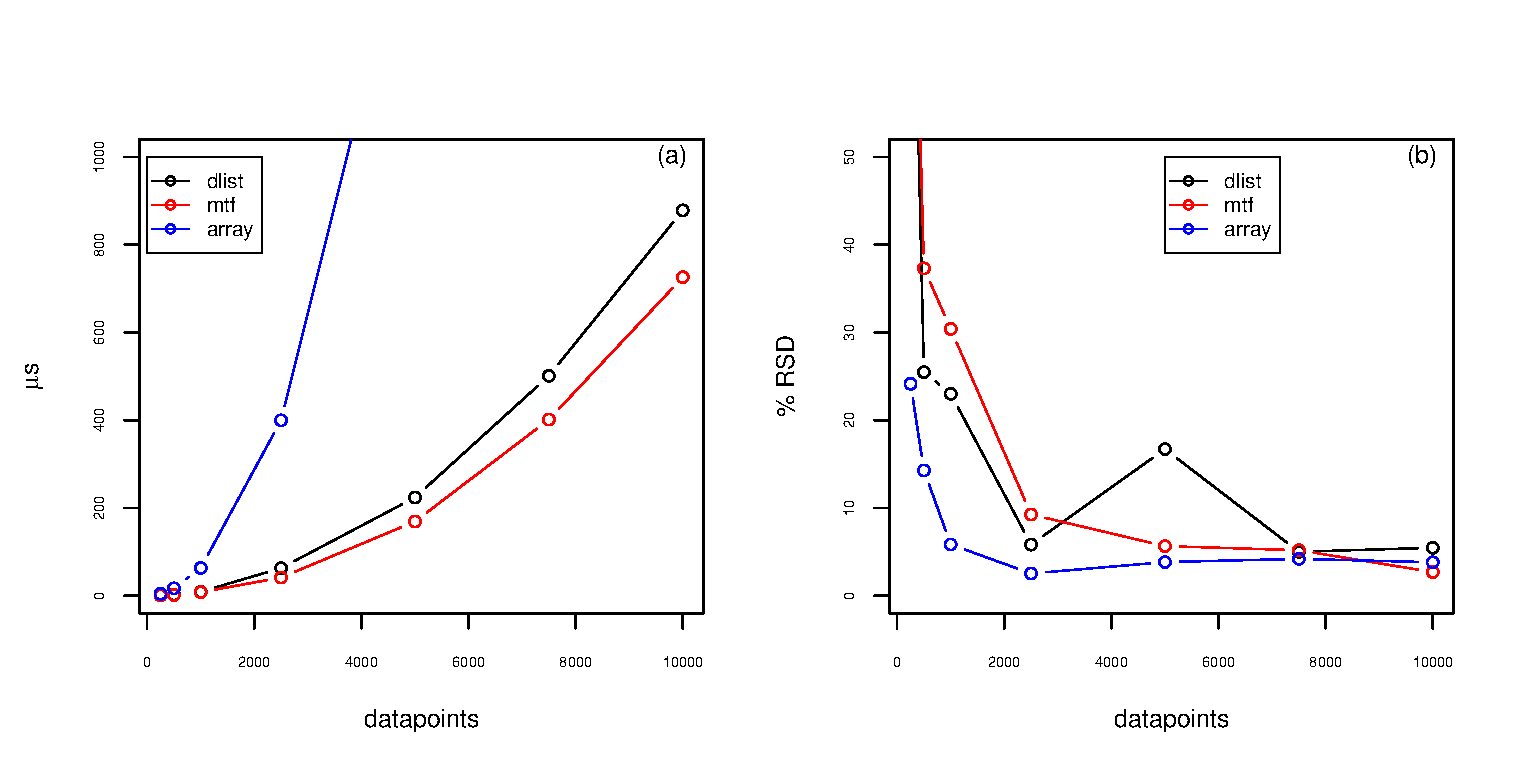
\includegraphics[width=\textwidth]{figures/fig5.eps}
\caption{\textit{Figure 5a, shows the times for the \textbf{`Removal'}
    benchmark. Figure 5b shows the RSD's from the measurments in figure 5a. n=10.}}
\end{figure}

\begin{figure}[H] 
\centering 
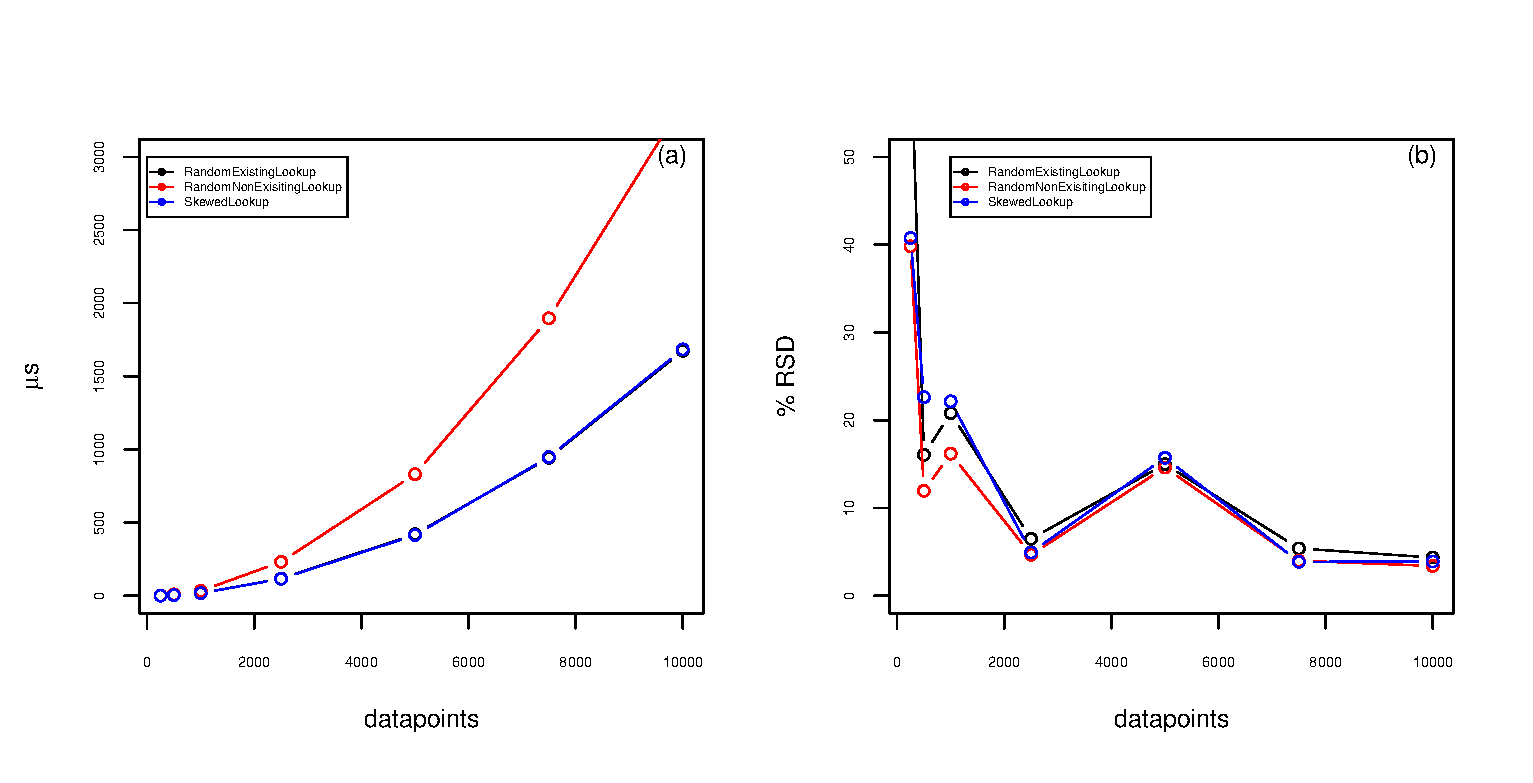
\includegraphics[width=\textwidth]{figures/fig6.eps}
\caption{\textit{Figure 6a, shows the times for the \textbf{`Random Existing
    Lookup'}, \textbf{`Random Non-Exisiting Lookup'} and
  \textbf{`Skewed Lookup'} benchmark of the datatype \textbf{`dlist'}. Figure 6b shows the RSD's from the measurments
in figure 6a. n=10.}}
\end{figure}

\begin{figure}[H] 
\centering 
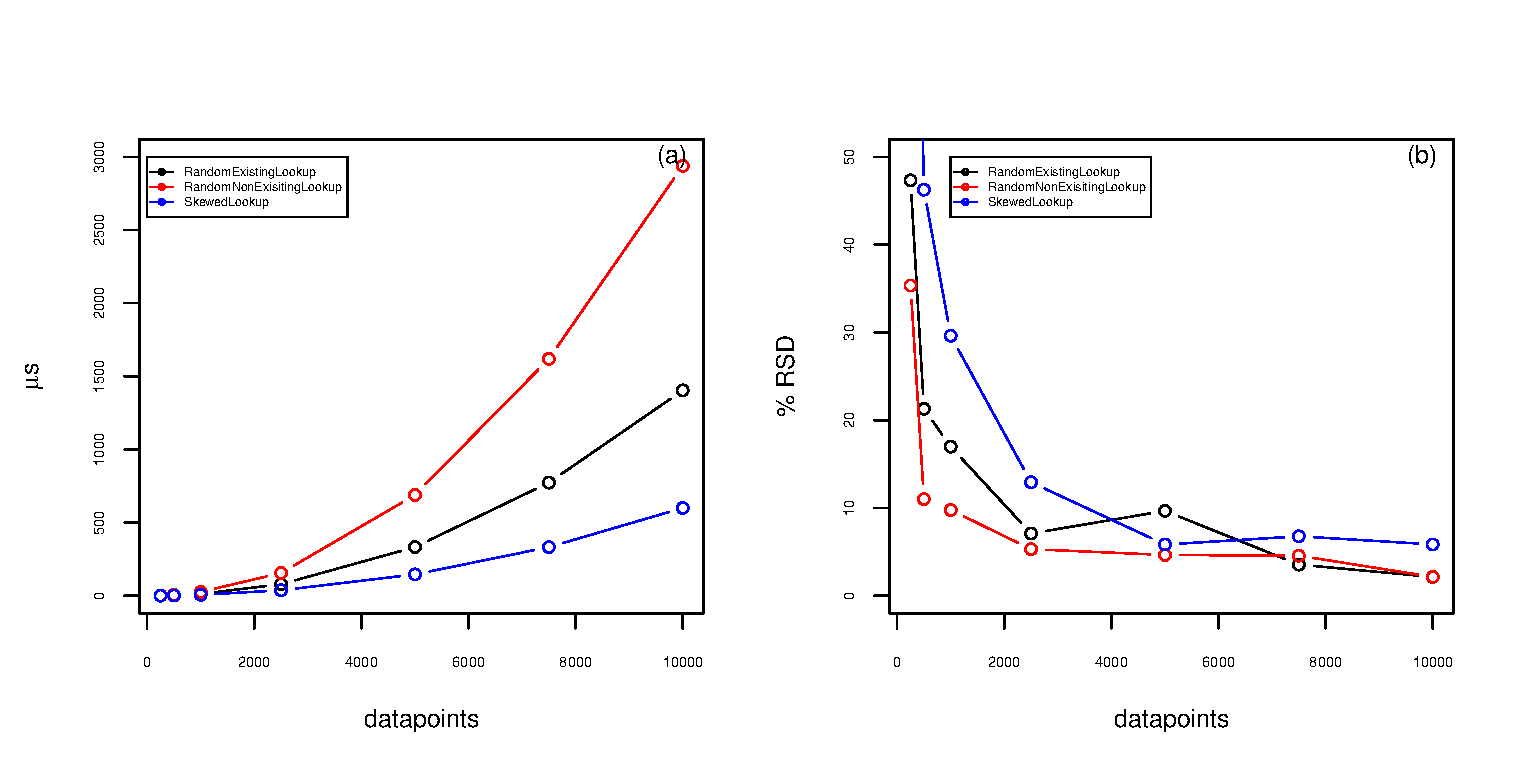
\includegraphics[width=\textwidth]{figures/fig7.eps}
\caption{\textit{Figure 7a, shows the times for the \textbf{`Random Existing
    Lookup'}, \textbf{`Random Non-Exisiting Lookup'} and
  \textbf{`Skewed Lookup'} benchmark of the datatype \textbf{`mtf'}. Figure 7b shows the RSD's from the measurments
in figure 7a. n=10.}}
\end{figure}

\begin{figure}[H] 
\centering 
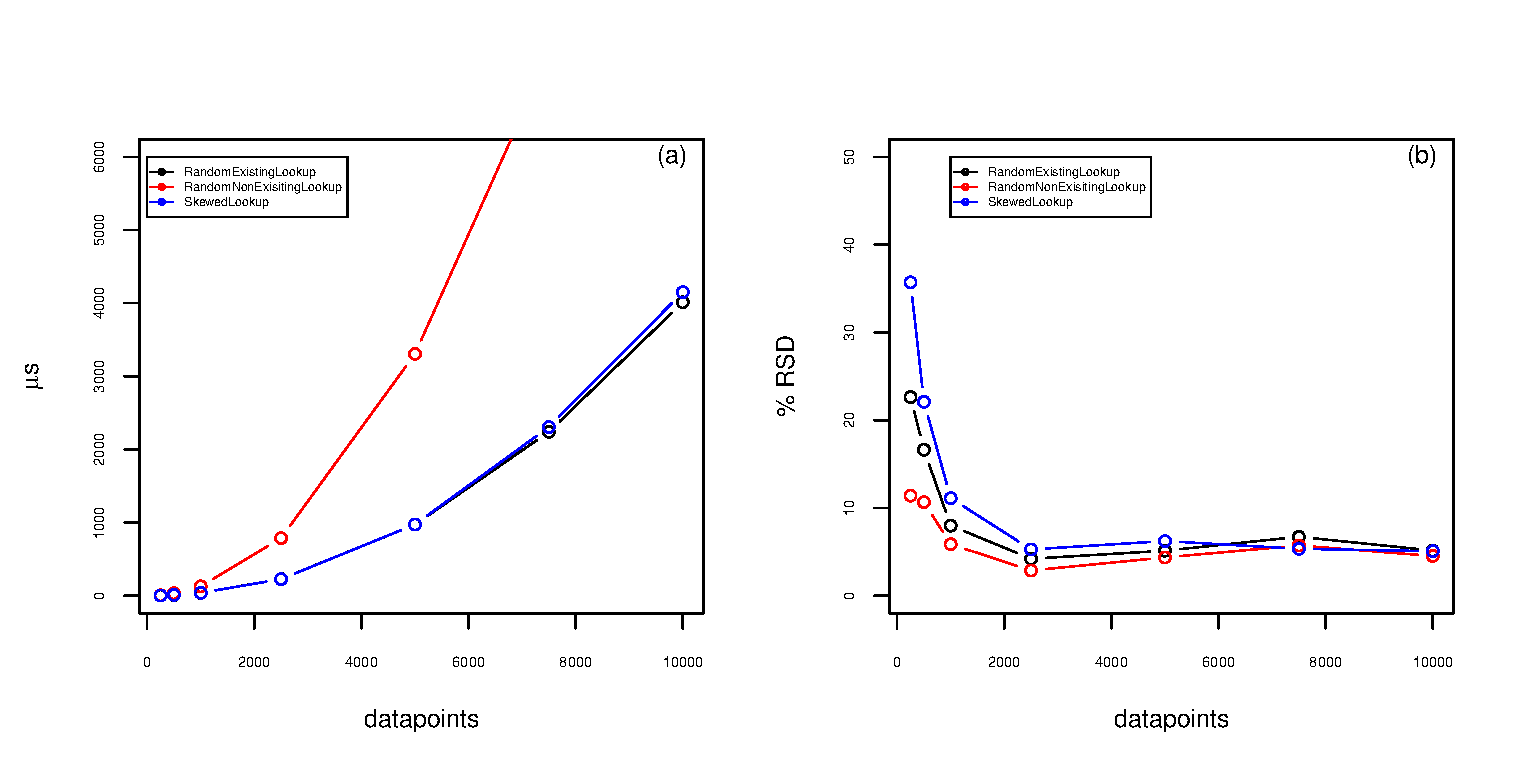
\includegraphics[width=\textwidth]{figures/fig8.eps}
\caption{\textit{Figure 8a, shows the times for the \textbf{`Random Existing
    Lookup'}, \textbf{`Random Non-Exisiting Lookup'} and
  \textbf{`Skewed Lookup'} benchmark of the datatype \textbf{`array'}. Figure 8b shows the RSD's from the measurments
in figure 8a. n=10.}}
\end{figure}


\section{Discussion}
Analysis of the results (1-3 pages). Flowing text. Shall answer at
least the following questions:
Which datatype was fastest, which (dis)advantages do the different
tabeltypes have? Reason for one advantage why the other implementation
don't offer it. Reasoning about dynamic/static implementation. If
done, reason why the direct indexing table is so fast.

\addcontentsline{toc}{section}{\refname}
\bibliography{references}

\end{document}
